% VLDB template version of 2020-08-03 enhances the ACM template, version 1.7.0:
% https://www.acm.org/publications/proceedings-template
% The ACM Latex guide provides further information about the ACM template

\documentclass[sigconf, nonacm]{acmart}

\usepackage{graphicx}
\usepackage{subcaption}

\newtheorem{theorem}{Theorem}
\newtheorem{example}{Example}
%% The following content must be adapted for the final version
% paper-specific
\newcommand\vldbdoi{XX.XX/XXX.XX}
\newcommand\vldbpages{XXX-XXX}
% issue-specific
\newcommand\vldbvolume{14}
\newcommand\vldbissue{1}
\newcommand\vldbyear{2020}
% should be fine as it is
\newcommand\vldbauthors{\authors}
\newcommand\vldbtitle{\shorttitle} 
% leave empty if no availability url should be set
\newcommand\vldbavailabilityurl{URL_TO_YOUR_ARTIFACTS}
% whether page numbers should be shown or not, use 'plain' for review versions, 'empty' for camera ready
\newcommand\vldbpagestyle{plain} 

\begin{document}
\title{Converged Optimizer for Efficient Join Order Optimization}

%%
%% The "author" command and its associated commands are used to define the authors and their affiliations.
%\author{Ben Trovato}
%\affiliation{%
%  \institution{Institute for Clarity in Documentation}
%  \streetaddress{P.O. Box 1212}
%  \city{Dublin}
%  \state{Ireland}
%  \postcode{43017-6221}
%}
%\email{trovato@corporation.com}


%%
%% The abstract is a short summary of the work to be presented in the
%% article.
\begin{abstract}

\end{abstract}

\maketitle

\section{Motivation}
\label{sec:motivation}
With the fast development and numerous usage of graph databases, graphs have been widely used in various fields to model data, such as the transportation networks, social networks, and financial systems.
Since graphs have obtain more attention in both the industrial and academic areas, SQL/PGQ has added the semantics about graphs into the standard.
For graphs, pattern matching is a common and crucial problem in both real-world and industrial applications, and it is reasonable to provide relational database the capability of efficienly dealing with the pattern matching problem.
Regarding the grammar of SQL/PGQ, users can conduct pattern matching by specifying paths in the pattern graph.
By default, pattern matching in SQL/PGQ indicates homomorphism pattern matching, and such pattern matching problems can be solved by multiple joins on tables.
Example \ref{example:intro} illustrates the idea of solving graph queries expressed with SQL/PGQ by multiple-joins.

\begin{figure*}
    \centering
    \begin{subfigure}[b]{0.4\linewidth}
        \centering
        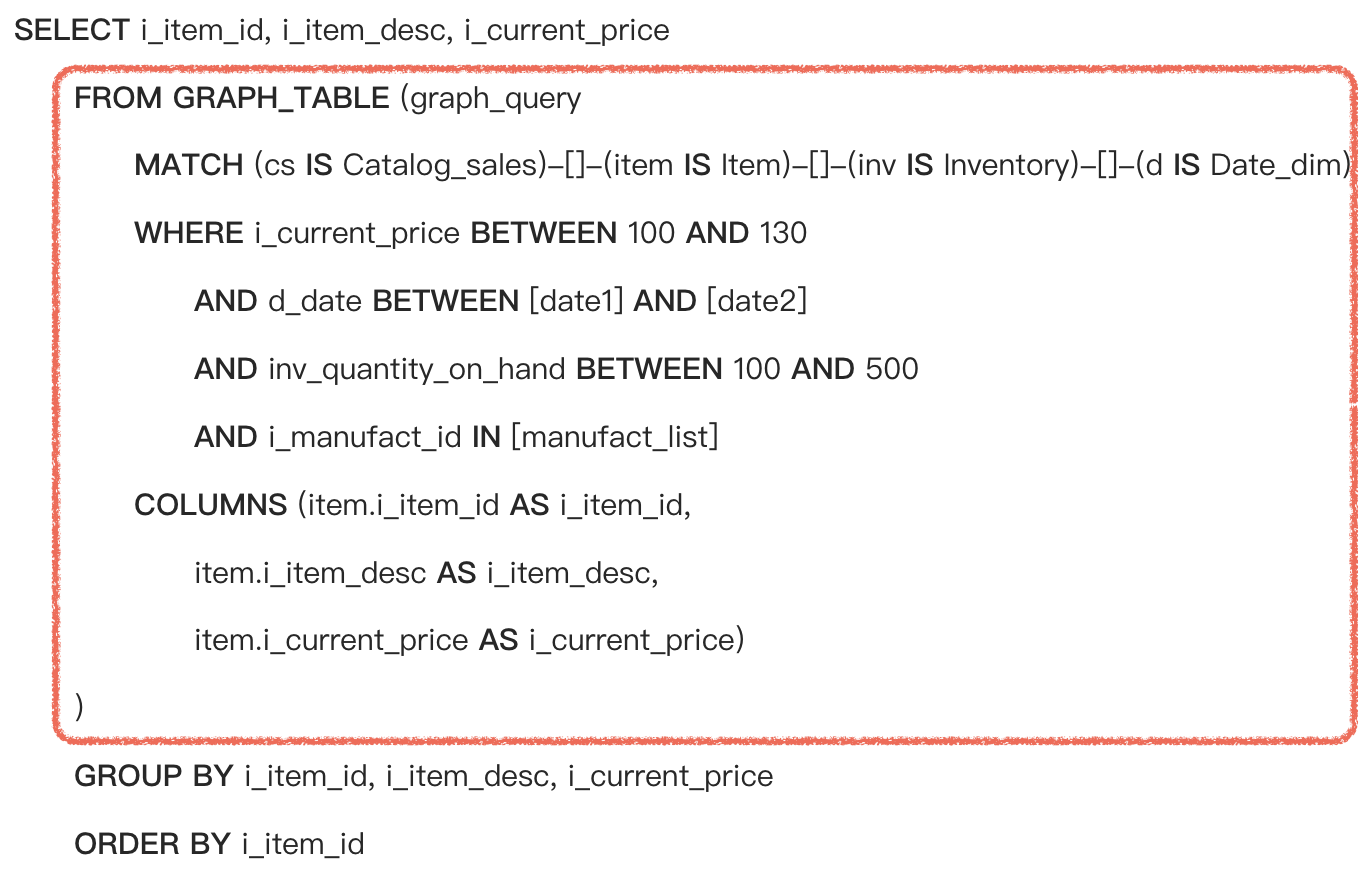
\includegraphics[width=\linewidth]{./figures/intro-select-convert.png}
        \caption{The SQL/PGQ query corresponding to Fig.~\ref{fig:intro-graph-query}.}
        \label{fig:intro-select-convert}
    \end{subfigure}
    \begin{subfigure}[b]{0.3\linewidth}
        \centering
        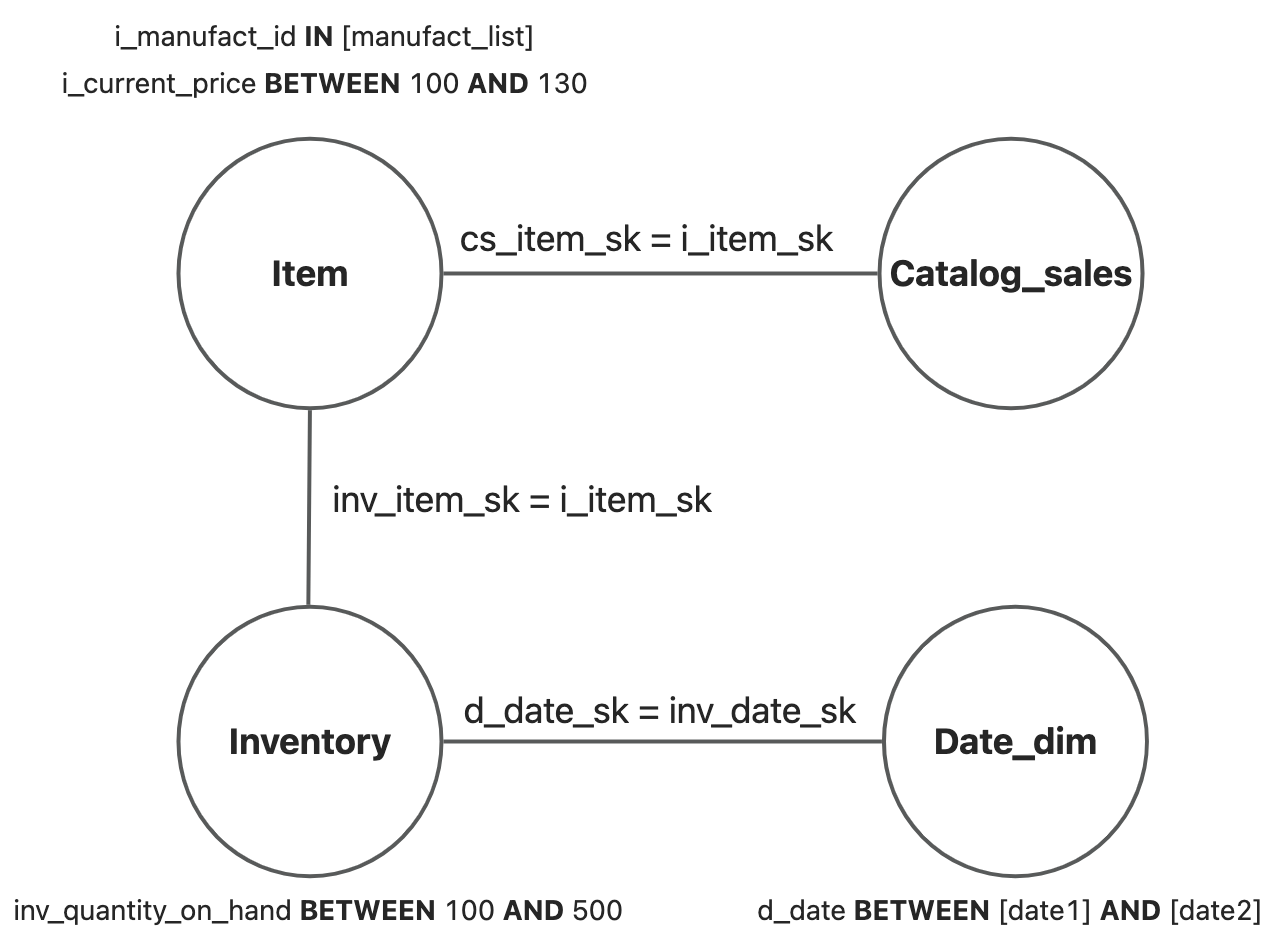
\includegraphics[width=\linewidth]{./figures/intro-graph-query.png}
        \caption{The pattern graph corresponding to the multiple-join in query \#37.}
        \label{fig:intro-graph-query}
    \end{subfigure}
    \begin{subfigure}[b]{0.25\linewidth}
        \centering
        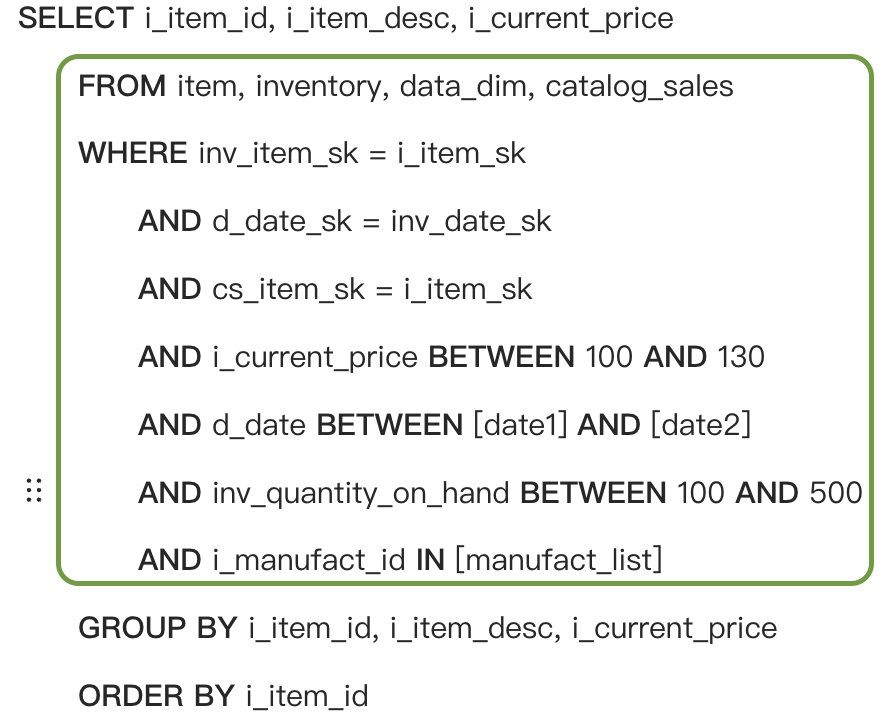
\includegraphics[width=\linewidth]{./figures/intro-select.png}
        \caption{Query \#37 of TPC-DS.}
        \label{fig:intro-tpcds-query}
    \end{subfigure}
    \caption{An example of solve graph queries expressed with SQL/PGQ by multiple-joins.}
    \label{fig:intro-example}
\end{figure*}

\begin{example}
\label{example:intro}
As shown in Fig.~\ref{fig:intro-example}, an example of transformation from SQL/PGQ queries to SQL queries is presented.
In detail, Fig.~\ref{fig:intro-select-convert} queries for the items, item descriptions, and current prices of these items during time period between date1 and date2, where the prices of the items should be between 100 and 130, the quantity on-hand should be between 100 and 500, and the manufact should be in the specified manufact list.

Specifically, the clause in the red rectangle specifies a pattern matching task, where the pattern graph is as shown in Fig.~\ref{fig:intro-graph-query}.
It is clear that such a pattern matching task can also be expressed with SQL and solved by multiple-joins.
The corresponding SQL query is shown in Fig.~\ref{fig:intro-tpcds-query}, and the clause in the green rectangle expresses the multiple-join used to solve the problem of pattern matching.
In fact, this SQL query is actually query \#37 in TPC-DS.
\end{example}

However, as stated in the previous literatures, the join order can influence the efficiency of queries significantly.
Specifically, querying with a plan with a good join order can be more than an order of magnitude faster than that with a bad join order.
Therefore, the join order optimization problem (abbr.~JOOP) becomes more important and it is urgent to design efficient methods for JOOP.
Many strategies have been proposed in the previous studies. 
The methods used to solve JOOP are called the join order optimizers (abbr.~JOPTs).
% For simplicity, the segment of a optimizer, which is used to optimize the join order, is called the JOO-optimizer in this paper.
Given a SQL/PGQ query with pattern matching, the existing work can be mainly categorized into two types regarding the ways they optimize the join order, i.e., translation-based JOPTs and Index-based JOPTs.

%However, although the relations and graphs are combined in the language levels as shown in SQL/PQL, they are still far from fully integrated in real-world applications, and the features of relations and are graphs are not exploited completely.
%For instance, relational optimizer and graph optimizer are hot and important topics in recent years, and the integration of them are not deeply studied yet. 
%In this paper, we focus on the problem of achieving better performances on query optimization by leveraging both the features of relational optimizers and graph optimizers.
%There are already many studies about relational optimizers and graph optimizers, and some existing works study the problem of involving the graph optimizer in the relational optimizer.
%These works can be categorized into two types, i.e., translation-based optimizer and hybrid optimizer.

\textbf{Translation-based JOPTs} translate the SQL/PGQ queries into relational queries, and then utilize the techniques of relational optimizers to optimize the translated query and find the optimal join order. 
A typical example is Apache/Age. 
Apache/Age translates the openCypher queries to relational queries and process the query with PostgreSQL relational database management system.
This type of methods process the JOO problem with relational query optimizers, which have been widely studied for a long time.

\textbf{Index-based JOPTs} combine the join order optimization techniques of relational optimizers and graph optimizers into a index-based JOPT.
Then, this optimizer can optimize graph query with the techniques of graph optimizers, and optimize relational queries with the techniques of relational optimizers.
In this way, the graph features (e.g., the neighborhood information) can be exploited, and the benefits of both relations and graphs can be leveraged. 
Normally, graph optimizers are involved into relational databases to combine the generate the index-based JOPTs.
In index-based JOPTs, to exploit the techniques of graph optimizers, graph indices need to be built, and sometimes graph views are also necessary to be constructed. 
A example of index-based JOPTs is that in GrainDB \cite{graindb}.
GrainDB is a relational database developed based on DuckDB.
It designs RID (Row ID) index to store the adjacent edges and one-hop neighbors of vertices.
Then, the results of several joins operators can be obtained by visiting the RID index once, and the efficiency of multiple join can be improved.


It is clear that index-based JOPTs can have better performances than the translation-based JOPTs.
The reason is that the index-based JOPTs can exert the capabilities of the existing studies w.r.t.~both relational optimizers and graph optimizers.
However, since the translation-based JOPTs translate graph queries into relational queries, they have the same power as relational optimizers in terms of join order optimization.
Therefore, the translation-based JOPTs actually only utilize the optimization of the relational optimizer, and the benefits of graph optimizers are hardly exploited.
However, the existing index-based JOPTs only make the process of getting neighbors of vertices and getting adjacent vertices of edges conveniently.
The process of optimization is not adjusted correspondingly, and the optimial plan are probably missed.

In this paper, we propose to design a converged JOPT, which integrates the relational optimizer and graph optimizer more deeply and evaluates the cost of operators more accurately. 
To design such a converged JOPT, there are mainly two challenges.

\textbf{Challenge 1: How to reduce the complexity of optimization}. 
For a relational optimizer like calcite, all the related tables are involved in the process of optimization, and different orders of joining these tables are traversed.
Besides, the physical implementations of operators are varied (e.g., merge join and hash join), and the cost of using different physical implementations should also be tried.
Therefore, the process of optimization and finding the best physical plan is time-consuming.
Then, after the JOPT from a relational optimzier is combined with the techniques in graph optimizers, the obtained JOPT can be more complex to conduct optimization.
Thus, it is necessary to design the JOPT efficiently to reduce the time complexity of optimization.


\textbf{Challenge 2. How to find a better plan when relational and graph optimizers are regarded together}.
Given a relational database, after the graph indices are built int it and graph views are constructed, some joins in a multiple join can be performed more efficiently, makeing the time cost reduce significantly.
For example, given three tables V1, E, and V2, suppose these three tables are joined (i.e., V1 $\bowtie$ E $\bowtie$ V2).
Then, if the tuples in V1 and V2 represent vertices in a graph, and the tuples in E represent edges in the graph, such a join means to find the one-hop neighbors of the vertices in V1.
Im a graph index (which is also a table), we can record the adjacent edges of the vertices in V1, and the process of joining V1 and E can be accelerated.
Besides, we can also record the neighbors of the vertices in V1, and then the neigbors of V1 can be obtained more easily with the index.
Clearly, the cost of V1 $\bowtie$ E $\bowtie$ V2 with the graph index is much smaller than the cost without the graph index.
Therefore, in a converged JOPT, the cost of join operators should be analyzed more carefully for generating better plans.


To the best of our knowledge, the existing JOPTs do not address these two challenges very well.
For example, GRainDB (based on DuckDB) implements graph indices that record the neighbors of each vertex.
However, GRainDB still uses the join order optimization methods in DuckDB, which is designed regardless of the graph indices and graph optimizer.
After the optimal physical plan is generated, GRainDB replaces some join operators with new join operators using graph indices to accelerate the queries.
Note that, the complexity of optimization is not reduced (Challenge 1), and the cost estimation is inaccurate.
Besides, since graph indices are not considered in the process of optimiztion, the search space of physical plans is not complete, and the optimal plan may be overlooked (Challenge 2).

Therefore, we tend to discover a better way to integrate the intelligence of join order optimziation in both relational optimizer and graph optimizer, and address the two challenges efficienly.
In detail, our contributions in this paper are as follows:

(1) We solve the problem of JOOP by designing an efficient converged JOPT, which deeply integrates the techniques of relational optimizers and graph optimizers to deal with the queries meeting the requirements of SQL/PGQ.
Instead of translating subgraph matching into corresponding relational queries or simply building indices, we carefully leverage the capabilities of both relational and graph optimizer to deal with such queries more efficiently.

(2) GLogue is applied to optimize the graph queries and generate the optimial physical plan.
In GLogue, patterns can be entended or be joined together, and the cost is estimated according to the built graph indices.
Besides, GLogue is worst-case optimial, and acclerates the process of optimization by inducing edge tables with vertex tables, and exploiting symmetry-breaking.

(3) We analyze the time complexity of join order optimization with Calcite and with GLogue, respectively.
The theorems indicate that join order optimization with GLogue can be exponentially faster than that with Calcite.
This theoretically prove that the GLogue has much better performance in multiple join.

(4) Experimental results show that our optimizer has smaller time cost in optimization, and can generate better plans than DuckDB and GRainDB.


\section{Related Work}
\label{sec:related-work}
In this section, we first summarize the previous studies of join order optimization methods in relational optimizers and in graph optimizers, respectively.
Then, existing index-based JOPTs are introduced.
Since such methods can be categorized into two types, i.e., translation-based JOPTs and index-based JOPTs, the related work of them are presented respectively.

\subsection{Join Order Optimization in Relational JOPTs}
\label{sec:related-work:ropt}
Join order optimization in relational databases is a traditional topic and has attained substantial accomplishments.
Various JOPTs have been proposed to accelerate the process of optimization.
Ibaraki et al.~\cite{nested-tods-1984} propose that there are usually fewer than ten tables involved in a typical query, and deal with joins with nested-loops join.
Specifically, they prove the NP-complexity of the join order optimization problem, and design an efficient algorithm with a time complexity of $O(n^2logn)$ to optimize tree queries.
Then, Krishnamurthy et al.~\cite{optimize-nested-vldb-1986} optimize the algorithm, and propose an algorithm with time complexity of $O(N^2)$ by reusing the computation results.
Besides, the authors emphasize that since finding the optimal join order is a complex problem, it is more important to avoid the worst plan.
Moreover, Haffner et al.~\cite{astarjoin} convert the problem of join order optimization to the problem of finding shortest path on directed graphs, and solve the problem with the A* algorithm.
In details, four heuristics are designed to estimate the remaining cost.
Furthermore, Kossmann et al.~\cite{data-dependency-join} summarize the methods to optimize queries with data dependencies.
For example, given two tables $T_1$ and $T_2$, if the values of attribute $A_1$ on $T_1$ are unique, then the inner-join in queries like 
\begin{equation*}
    \text{SELECT}\hspace{.5em} T_2.A_2 \hspace{.5em}\text{FROM}\hspace{.5em} T_1, T_2 \hspace{.5em}\text{WHERE}\hspace{.5em} T_1.A_1 = T_2.A_2
\end{equation*}
may be converted into a semi-join, which is more efficient.


There are also some studies that try to find better plans with more accurate estimation of cardinalities.
Some researchers propose to estimate the number of cardinalities with sampling \cite{index-based-join-sampling,ripple-join,wanderjoin,index-based-join-sampling}.
Specifically, Li et al.~\cite{wanderjoin} present an unbiased estimator based on random walk to estimate the cardinalities.
Leis et al.~\cite{index-based-join-sampling} propose a cheap method, i.e., index-based join sampling, to improve the accuracy.
Some other researchers \cite{selinger,postgres-row-estimation} estimate the number of cardinalities by computing the selectivity of $A \bowtie_{A.col_1 = B.col_2} B$ as 
\begin{equation*}
    \frac{1}{max(DV(A.col_1), DV(B.col_2))},
\end{equation*}
where $DV(A.col_1)$ is the number of distinct values of $A.col_1$ in table $A$.
Besides, some studies estimate the number of cardinalities with histograms \cite{histogram,postgres-row-estimation}.
These methods split the values of a table column into several buckets to build a histogram, and assume that the values are uniformly distributed in each bucket.
Then, the cardinality is estimated by summing up the numbers of values in the related buckets.
Moreover, there are also some studies estimate cardinalities with learning-based methods \cite{learning-based-estimation-1,learning-based-estimation-2,learning-based-estimation-3,learning-based-estimation-4}.


\subsection{Join Order Optimization in Graph JOPTs}
\label{sec:related-work:gopt}
When the subgraph matching problem is solved by the join of tables representing vertices and edges, graph optimizers are considered to deal with JOOP as well.

Recently, some studies have been conducted to estimate cardinalities in the process of subgraph matching.
In detail, 
C-Set \cite{cset} decomposes the query graph and the data graph into star-shaped subgraphs, and constructs characteristic sets to estimate.
AutoMine \cite{AutoMine} proposes to estimate the cost of a plan for subgraph matching with the number of iterations in the nested loop.
DecoMine \cite{DecoMine} improves the method of AutoMine and presents an approximate-mining based cost model to estimate the costs of nested loops.
Then, DecoMine finds the optimal abstract syntex tree with the smallest cost.
GLogS \cite{GLogS} proposes a graph optimizer named GLogue to search for the optimal plan.
In GLogue, an edge can represent a binary join or a subtask of an extension, and please note that an extension can be regarded as a set of joins.
GLogue computes the optimal plan in a bottom-up manner, and can efficiently obtain a worst-case optimal plan.
Besides, G-CARE \cite{gcare} compares the performances of different methods for cardinality estimation.



\subsection{Join Order Optimization in Relational-Graph JOPTs}
\label{sec:related-work:ropt-gopt}
The existing works about integrating relational optimizers and graph optimizers can be roughly categorized into two classes, i.e., translation-based JOPTs and index-based JOPTs.

In terms of translation-based JOPTs, Apache/Age \cite{apache-age} is a typical work.
Apache/Age is an extension of PostgreSQL, and it provides the ability to handle hybrid queries including openCypher and SQL.
In detail, after a graph is created, a namespace with the same name as the graph is created, and the vertices and edges are stored in corresponding tables in the namespace.
When a query with both openCypher and SQL statements is conducted, Apache/Age transforms the openCypher statements and convert the operators to those in PostgreSQL (e.g., join), and then the query is solved by PostgreSQL.
It seems that Apache/Age is like a syntactic sugar, and the advantanges of graphs and graph optimizers are not utilized.

In terms of index-based JOPTs, such methods build graph indices or graph views on the relational databases, and attempt to accelerate queries with the indices.
GRFusion \cite{GRFusion} builds a graph view in main-memory based on the relational tables, and supports queries on both tables and graph views.
Then, some relational joins can be replaced with graph traversals, and some graph-level optimizations can be applied.
GQ-Fast \cite{gqfast} is proposed to deal with relationship queries, and works accompanying with traditional relational databases.
Specifically, in GQ-Fast, indices with lookup data structure are built to accelerate.
Given a SQL query, GQ-Fast generates physical plans by transforming relationship query normalized algebra expressions with a Physical-plan Producer, and more optimizations for the plans are necessary.
GrainDB \cite{graindb} builds RID indices, and presents two new join methods (i.e., sip-join and merged-sip-join) that can get the adjacent edges and one-hop neighbors of vertices with RID indices.
Based on these join methods, in some settings, the cost of multiple joins can be reduced significantly.
However, GrainDB inherits the optimizer of DuckDB, and replaces some joins with sip-joins and merged-sip-joins.
Therefore, cost estimation in the optimizer may not be optimal and the best plan can be missed.


\section{Preliminaries}
\label{sec:preliminaries}



\begin{figure*}
    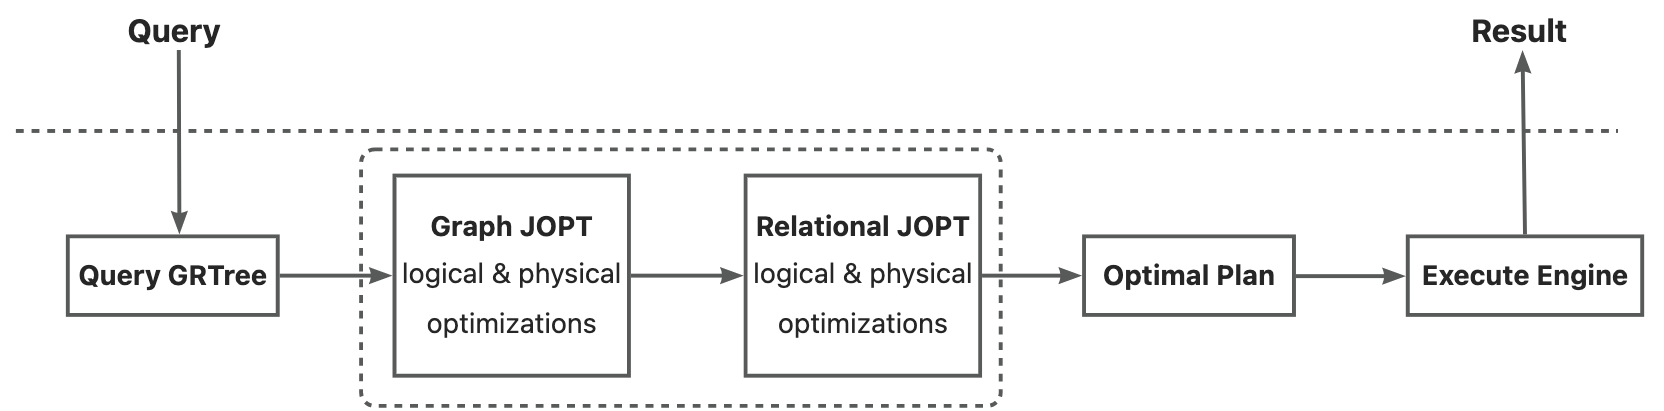
\includegraphics[width=.8\textwidth]{figures/dataflow.png}
    \caption{The dataflow of the converged JOPT.}
    \label{fig:dataflow}
\end{figure*}

\section{Overview of the Converged JOPT}
\label{sec:overview}
For the converged JOPT, it integrates the capabilities of both the relational and graph databases.
The dataflow of the converged JOPT is shown in Fig.~\ref{fig:dataflow}.
In detail, with the query statement provided by the user, a query tree is first constructed.
Since both relational operators and graph operators can be used as tree nodes, the query trees generated here is different from those generated in relational databases.
Specifically, the query trees generated for the converged JOPT are called the query graph-relational-trees (abbr.~the query GRTrees).
An example of a query GRTree is shown in Fig.~\ref{fig:query-grtree-pattern}.
Given a query as follows:
\begin{equation*}
    \begin{split}
        & \text{SELECT}\hspace{.5em} * \\ 
        & \hspace{.5em}\text{FROM}\hspace{.5em} graph\_table (graph\_pg \\
        & match \\
        & (inv is Inv) -[]- (d is Date), \\
        & (inv)-[]-(item is Item)-[]-(cat is Catalog)-[]-(inv) \\
        & columns (p1.name as person1,\\
        &     p2.name as person2)\\
        & );
    \end{split}
\end{equation*}
It means to conduct pattern matching with the pattern graph shown in Fig.~\ref{fig:query-grtree-pattern}.
A possible query GRTree is shown in Fig.~\ref{fig:query-grtree}.
Please note that operators \textbf{Expand}, \textbf{GetV}, and \textbf{Intersect} are not defined in the query trees of relational databases, and they are special for graph JOPTs.
These three operators are presented in GLogue \cite{GLogS}, and are applied to get the adjacent vertices of edges, or the common neighbors of vertices.
To be specific, \textbf{Expand($l_s$->$l_t$)} gets the edges from vertices labeled \textit{$l_s$} to vertices labeled \textit{$l_t$}.
For example, as shown in Fig.~\ref{fig:query-grtree}, by expanding from a vertex labeled \textit{Catalog} with \textbf{Expand(\textit{Catalog}->\textit{Item})}, edges from \textit{Catalog} to \textit{Item} are obtained.
Similarly, edges from \textit{Inv} to \textit{Item} are also obtained with \textbf{Expand(\textit{Inv}->\textit{Item})}.
\textbf{GetV($l_t$)} is usually used after an \textbf{Expand} operator, and it gets the destination vertices of the edges obtained with \textbf{Expand}. 
\textbf{Intersect()} gets the intersection of several vertex sets to obtain the common neighbors.
For example, with the \textbf{Intersect()} operator in Fig.~\ref{fig:query-grtree}, the common neighbors of a vertex labeled \textit{Catalog} and a vertex labeled \textit{Inv} is obtained.

\begin{example}
Fig.~\ref{fig:query-grtree} and Fig.~\ref{fig:query-grtree-2} show two possible query GRTrees (i.e., $\text{GRT}_1$ and $\text{GRT}_2$) w.r.t.~the pattern in Fig.~\ref{fig:query-grtree-pattern}.
In detail, $\text{GRT}_1$ first finds paths matching the pattern \textit{Date}-\textit{Inv}-\textit{Catalog}, and then find the common neighbors of the vertices labeled \textit{Inv} and \textit{Catalog}, respectively.
Meanwhile, $\text{GRT}_2$ conducts pattern matching with equal-joins.
$\text{GRT}_2$ first joins the paths obtained by pattern matching w.r.t.~\textit{Item}-\textit{Inv} and \textit{Item}-\textit{Catalog}, respectively.
Then, equal-joins are conducted again between the results and paths labeled \textit{Inv}-\textit{Date}.
\end{example}

\begin{figure*}
    \centering
    \begin{subfigure}[b]{0.15\linewidth}
        \centering
        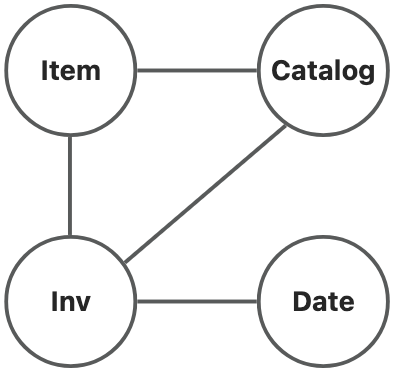
\includegraphics[width=\linewidth]{./figures/query-grtree-pattern.png}
        \caption{The queried pattern.}
        \label{fig:query-grtree-pattern}
    \end{subfigure}
    \begin{subfigure}[b]{0.35\linewidth}
        \centering
        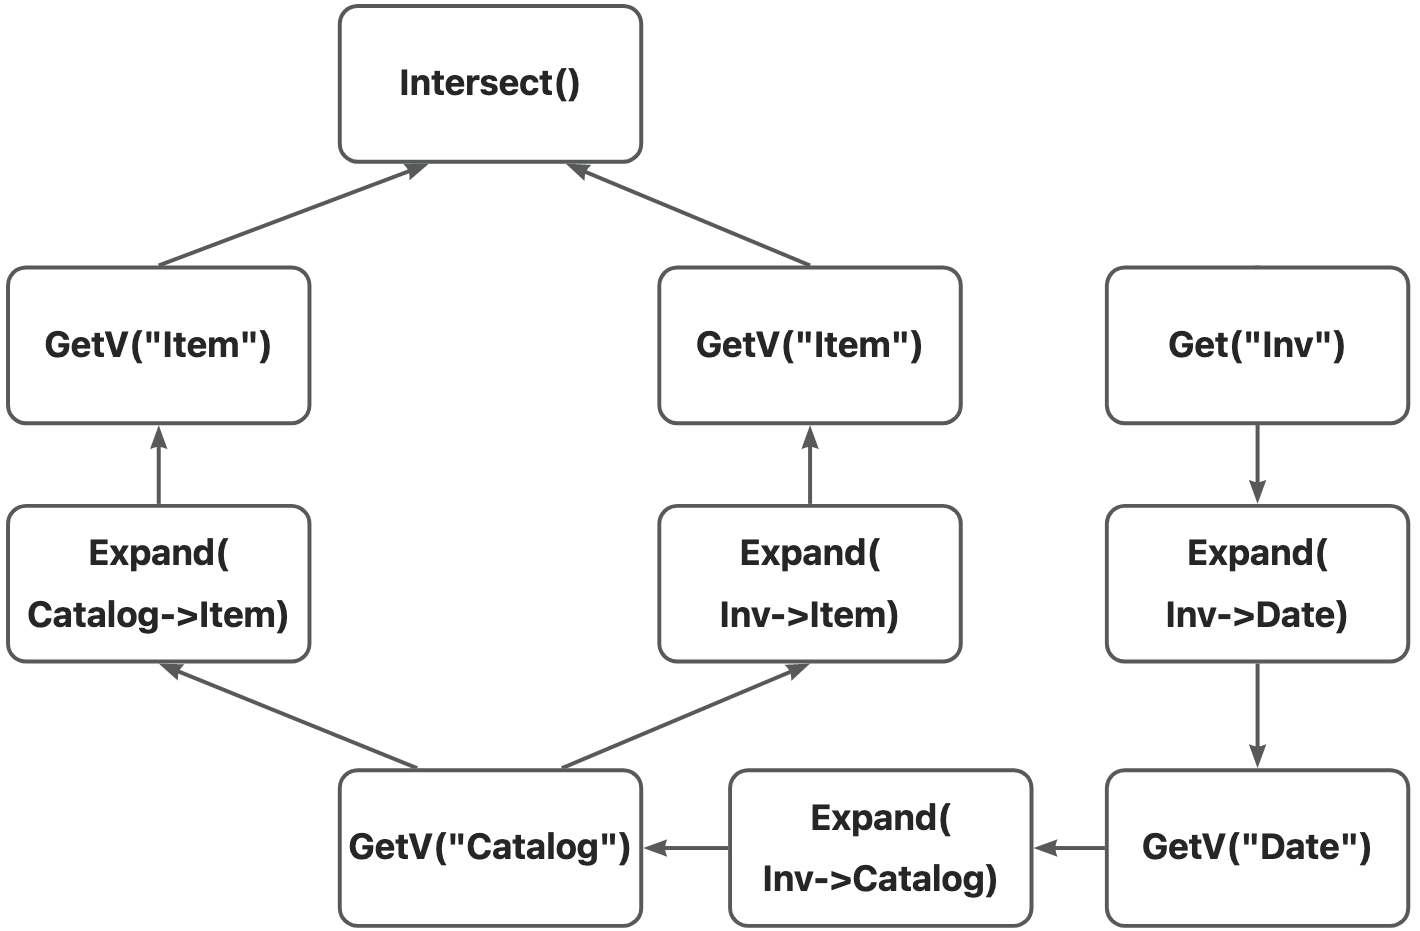
\includegraphics[width=\linewidth]{./figures/query-grtree.png}
        \caption{The query GRTree $\text{GRT}_1$.}
        \label{fig:query-grtree}
    \end{subfigure}
    \begin{subfigure}[b]{0.3\linewidth}
        \centering
        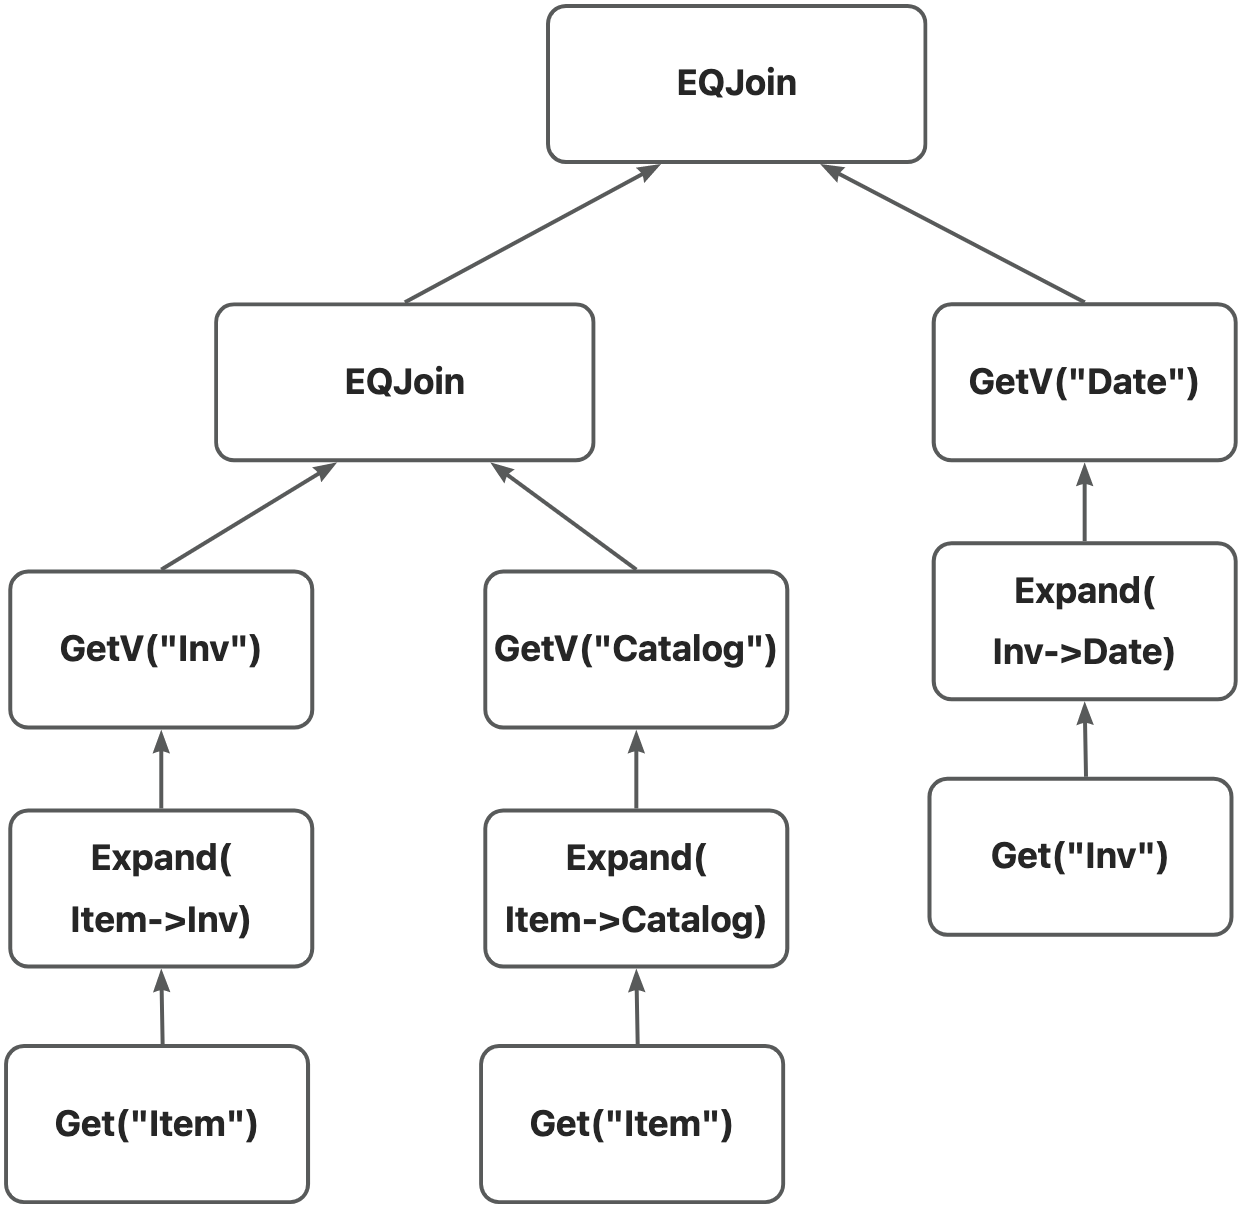
\includegraphics[width=\linewidth]{./figures/query-grtree-2.png}
        \caption{The query GRTree $\text{GRT}_2$.}
        \label{fig:query-grtree-2}
    \end{subfigure}
    \caption{An example of query GRTree.}
    \label{fig:query-grtree-example}
\end{figure*}

Then, the converged JOPT optimizes the query GRTree to generate the optimal plan.
In detail, the tables that can represent vertices and edges are first distinguished, and the graph JOPT optimizes the join order among these tables.
The join of these tables can produce an intermediate table, which is denoted as $T_{inter}$.
Then, for the tables that cannot represent vertices and edges, the relational JOPT optimizes the join order among these tables together with $T_{inter}$, and generates the optimial plan.
Finally, the execute engine queries with the plan, and returns the results to the user.



\section{Theoretical Analysis about the Superiority of the Converged JOPT}
\label{sec:theoretical-analysis}

In this section, we prove that the converged JOPT is faster in join order optimization than the well-studied relational JOPTs by analyzing their complexities respectively.
As one of the most widely adopted optimizers for relational databases, we use Calcite \cite{calcite,columbia} as a representative of relational JOPTs and analyze its efficiency of join order optimization.
For the converged JOPT, we use GLogue \cite{GLogS} as the graph JOPT, and integrate it with Calcite.

A more simple condition is first considered.
That is, all the tables in the query can represent vertices or edges.
Then, it is supposed that there are $n + m$ tables are joined together, where $n$ tables represent vertices while $m$ tables represent edges.
Suppose that there are $t$ implementation methods for join.
The complexities of optimizing the join order with Calcite and the converged JOPT are analyzed respectively as follows.
For simplicity, the time complexities are evaluated by the number of physical plans generated by the JOPTs.

\begin{theorem}
    \label{theorem:complexity-of-calcite}
    The time complexity of join order optimization with Calcite is at least $O(\frac{4^{m+n-1}}{m+n}t^{m+n-1})$.
\end{theorem}
\begin{proof}
    The $n + m$ tables joined together can form a graph, where the tables represent vertices in the graph, and if there is a join condition specifying the equivalence of two columns in two two tables, there is an edge between these two tables.
    Then, the complexity of join order optimization with Calcite can be estimated as the number of possible physical plans that can be generated.
    
    To avoid cross product, except for the first table, the selected tables to be be joined with the already chosen tables should be neighbors of the chosen tables in the graph.
    Therefore, the join order can be represented as a spanning tree in the graph.
    By computing the number of physical plans can be generated according to each spanning tree, the total number of physical plans can be obtained.
    However, same phyical plans may be obtained according to different spanning trees.
    For example, suppose a graph is a rectangle with four vertices and four edges.
    It may be constructed for a query like:
    \begin{equation*}
        \begin{split}
            \text{SELECT}\hspace{.5em} ... & \hspace{.5em}\text{FROM}\hspace{.5em} A, B, C, D \hspace{.5em}\text{WHERE}\hspace{.5em} A.1 = B.1 \\ 
            & \hspace{.5em}\text{AND}\hspace{.5em} B.2 = C.1 \hspace{.5em}\text{AND}\hspace{.5em} C.2 = D.1 \hspace{.5em}\text{AND}\hspace{.5em} D.2 = A.2. 
        \end{split}
    \end{equation*}
    Then, the spanning tree with edges \{AB, BC, CD\} and the one with edges \{AB, BC, AD\} can generate same physical plans.
    Consequently, the summation of the number of physical plans corresponding to all the spanning trees is larger than the actual number of physical plans.
    In this proof, we compute the number of physical plans for one spanning tree, and this number is the lower bound of the number of physical plans that can be generated.

    Given a spanning tree with $k$ edges (i.e., $k+1$ vertices representing tables) and only one leaf node, the number of logical plans corresponding to the spanning tree is roughly
    \begin{equation*}
        \begin{split}
            c(k) & = 2 * (c(0)c(k-1) + c(1)c(k-2) + \cdots + c(k-1)c(0)) \\
            & = 2\Sigma_{i=0}^{i=k-1}c(i)c(k-1-i), \\
            & \text{where } c(0) = 1.
        \end{split}
    \end{equation*}
    With the generating function, it is obtained that 
    \begin{equation*}
        c(k) = \frac{2^k}{k+1}C(2k, k).
    \end{equation*}
    Since $k$ is the number of edges, and $k = m + n - 1$ in the spanning tree.
    Thus, the number of logical plans w.r.t.~a spanning tree is 
    \begin{equation*}
        \frac{2^{m+n-1}}{m+n}C(2m+2n-2, m+n-1) \geq \frac{4^{m+n-1}}{m+n}.
    \end{equation*}
   Then, the number of physical plans is at least $\frac{4^{m+n-1}}{m+n}t^{m+n-1}$, so is the complexity of join order optimization with Calcite.
   
   In conclusion, Theorem \ref{theorem:complexity-of-calcite} is correct.
\end{proof}

\begin{lemma}
    \label{lemma:upper-bound-of-calcite}
    Given $n$ tables, the time complexity of join order optimization with Calcite has an upper bound of $O(\frac{(2n-2)!}{(n-1)!}t^{n-1})$.
\end{lemma}
\begin{proof}
    The upper bound of the time complexity of join order optimization is achieved when there is a condition between any two of the $n$ tables.
    Because at that time, the tables can be joined in any order.

    Since each join order corresponds to a full binary tree with $2n-1$ nodes, the problem is to count the number of possible full binary trees.
    Similar to Catalan number, the number of full binary trees is $O(C(2n-2, n-1) - C(2n-2, n))$.
    For each full binary tree, there are $n!$ ways to set the leaf nodes. 
    Then, the number of generated physical plans is $O(\frac{(2n-2)!}{(n-1)!}t^{n-1})$.
\end{proof}

\begin{theorem}
    \label{theorem:complexity-of-glogue}
    The time complexity of join order optimization with the converged JOPT is smaller than $3^n$ if all the tables participant in join can represent vertices or edges.
\end{theorem}
\begin{proof}
    Since the $n + m$ tables represent vertices and edges respectively and the join among them can be represented as a graph query, the converged JOPT optimizes the join order with the graph optimizer, i.e., GLogue.

    As GLogue ensures worst-case optimality and the considered patterns are all induced subgraphs, the time complexity of join order optimization with GLogue is not related to the number of edges (i.e., $m$).
    Because JOOP is reduced to a variant of shortest path problem, the time complexity of join order optimization is $O(\mathcal{E})$, where $\mathcal{E}$ is the number of edges in GLogue.
    In detail, 
    \begin{equation*}
        \begin{split}
            O(\mathcal{E}) & = C(n, n-1)*(2^{n-1}-1) + C(n, n-2) * (2^{n-2}- 1) \\
            & + \cdots + C(n, 1) * (2^1 - 1) \\
            & = 3^n - 2^{n+1} +1 \\
            & < 3^n.
        \end{split}
    \end{equation*}
    
    In conclusion, Theorem \ref{theorem:complexity-of-glogue} is correct.

\end{proof}

Based on the complexity analysis in Theorem \ref{theorem:complexity-of-calcite} and Theorem \ref{theorem:complexity-of-glogue}, it is found that when the tables represent vertices and edges, 
\begin{equation*}
    \begin{split}
        \frac{\text{Time Complexity of Calcite}}{\text{Time Complexity of the Converged JOPT}} & = \frac{\frac{4^{m+n-1}}{m+n}}{3^n}t^{m+n-1} \\
        & \geq 2^{m-3}(\frac{4}{3})^nt^{m+n-1}.
    \end{split}
\end{equation*}
Therefore, it suggests that the converged JOPT is exponentially faster than Calcite for graph-like join order optimization.
The results also indicates that integrating graph optimizers into relational optimizers can improve the efficiency of join order optimization significantly.


Then, if there are some tables that cannot represent vertices or edges, the order of such tables cannot be optimized with graph optimizers, and the comparion becomes more complicate.
For example, suppose five tables form a clique, and then these tables cannot be vertices or edges in a graph.
Specifically, according to the dataflow shown in Fig.~\ref{fig:dataflow}, the join order of these left tables are optimzed by relational optimizers such as Calcite.
Let the number of left tables be $s$, and together with the table obtained by the join of the tables optimized with graph optimizer, Calcite needs to optimize the join order among $s + 1$ tables.

When $s = 0$, all the tables represent vertices or edges, and the time complexity of the converged JOPT is exponentially smaller than that of Calcite as analyzed as above.

When $s = 1$, only one table (saying $T_1$) does not represent a vertex or an edge, and Calcite optimizes the join between two tables.
One of these two tables is $T_1$, and the other is the table obtained by the join of the tables optimized with graph optimizer.
Then, we have
\begin{equation*}
    \begin{split}
        \frac{\text{Time Complexity of Calcite}}{\text{Time Complexity of the Converged JOPT}} > \hspace{-12em} & \\
        & \frac{\frac{2^{m+n-1}}{m+n}C(2m+2n-2, m+n-1)t^{m + n - 1}}{3^{\hat{n}} + \frac{(2s)!}{(s)!}t^{s}} \\
        & = \frac{\frac{2^{m+n-1}}{m+n}C(2m+2n-2, m+n-1)t^{m + n - 1}}{3^{\hat{n}} + 2} >> 1,
    \end{split}
\end{equation*}
where $\hat{n}$ is the number of tables representing vertices.
It indicates the superiority of the converged JOPT.

When $s = m + n - 1$ or $p = m + n$, at most one table can represent vertices or edges, and the converged JOPT degenerates to Calcite, and has the same efficiency as it.
A typical example is when there is a condition between any two of these $m + n$ tables.

The results show that the converged JOPT is always superior to relational JOPTs.
To be more specific, we prove the superiority of the converged JOPT more theoretically.

\begin{lemma}
    \label{lemma:join-spliter}
    Let $\text{JN}_c(V_s)$ represent the number of possible physical plans of joining tables in table set $V_s$ with Calcite.
    Suppose $n$ tables (denoted as table set $V$) are joined, and $V = (V_1 - u) \cup V_2$, $V_1 \cap V_2 = \emptyset$.
    Specifically, $u \in V_1$ is a table representing the results of joining the tables in $V_2$.
    For each table $t_2 \in V_2$, if there is a join condition between $t_2$ and a table $v$ in $V_1$, the same join condition exists between $u$ and $v$.
    Then, we have $\text{JN}_c(V) \geq \text{JN}_c(V_1) * \text{JN}_c(V_2)$.
\end{lemma}
\begin{proof}
    For a physical plan generated by joining tables in $V_1$ (denoted as $p_1$) and a plan generated by joining tables in $V_2$ (denoted as $p_2$), by replacing $u$ in $p_1$ with $p_2$, we can generate a physical plan of joining tables in in $V$.
    Besides, since the tables in $p_1$ cannot be interchanged with tables in $p_2$, more physical plans can be generated by joining tables in $V$.
    In conclusion, we have $\text{JN}_c(V) \geq \text{JN}_c(V_1) * \text{JN}_c(V_2)$.
\end{proof}

\begin{theorem}
    \label{theorem:complexity-of-converged-jopt}
    The time complexity of join order optimization with the converged JOPT is always smaller than that with Calcite.
\end{theorem}
\begin{proof}
    Denote the set of tables that cannot represent vertices and edges by $S$.
    Besides, denote the set of tables that represent vertices and edges by $R$, and denote the table obtained by joining the tables in $R$ by $T_r$.
    Then, we have $S_r = S \cup T_r$.
    Moreover, let $s = |S|$ and $r = |R|$ represent the size of tables set $S$ and $R$, respectively, and let $s_v$ be the number of tables in $S$ representing vertices.
    Denote the number of possible physical plans of joining tables in $R$ with GLogue by $\text{JN}_g(R)$.
    
    Specifically, according to Theorem \ref{theorem:complexity-of-calcite} and Theorem \ref{theorem:complexity-of-glogue}, we have $\text{JN}_g(R) < 3^{s_v} \leq \frac{4^{r-1}}{r}t^{r-1} \leq \text{JN}_c(R)$.
    Note that $T_r$ corresponds to $u$ in Lemma \ref{lemma:join-spliter}.
    Based on Lemma \ref{lemma:join-spliter}, we have $\text{JN}_c(S \cup R) \geq \text{JN}_c(S_r) * \text{JN}_c(R) \geq \text{JN}_c(S_r) * \text{JN}_g(R)$.
    In conclusion, Theorem \ref{theorem:complexity-of-converged-jopt} is correct, and the converged JOPT always has smaller time complexity than Calcite.
\end{proof}

There are mainly three reasons contributing to the efficient performance of the converged JOPT:
(1) Different implementations of the join operators are not considered in the converged JOPT, because the neighbors of vertices can be efficiently accessed with the graph indices.
(2) In the converged JOPT, only the number of vertices influence the complexity of join order optimization, while the complexity is determined by both the numbers of vertices and edges in Calcite.
(3) The converged JOPT can take isomorphism into consideration in optimization and further reduce the search space, while Calcite does not consider optimization related to isomorphism.


\section{System Implementation}
\label{sec:system-implementation}


\section{Evaluation}
\label{sec:evaluation}


\section{Conclusions}
\label{sec:conclusions}


%\begin{acks}
% This work was supported by the [...] Research Fund of [...] (Number [...]). Additional funding was provided by [...] and [...]. We also thank [...] for contributing [...].
%\end{acks}

%\clearpage

\bibliographystyle{ACM-Reference-Format}
\bibliography{sample}

\end{document}
\endinput
